\documentclass[12pt, border=8pt]{standalone}
\usepackage{tikz}
\usepackage{amsmath, amssymb, bm}
\usepackage{xcolor}
\usepackage{booktabs}
\usetikzlibrary{positioning, arrows.meta, calc, fit, backgrounds, 3d}

\begin{document}


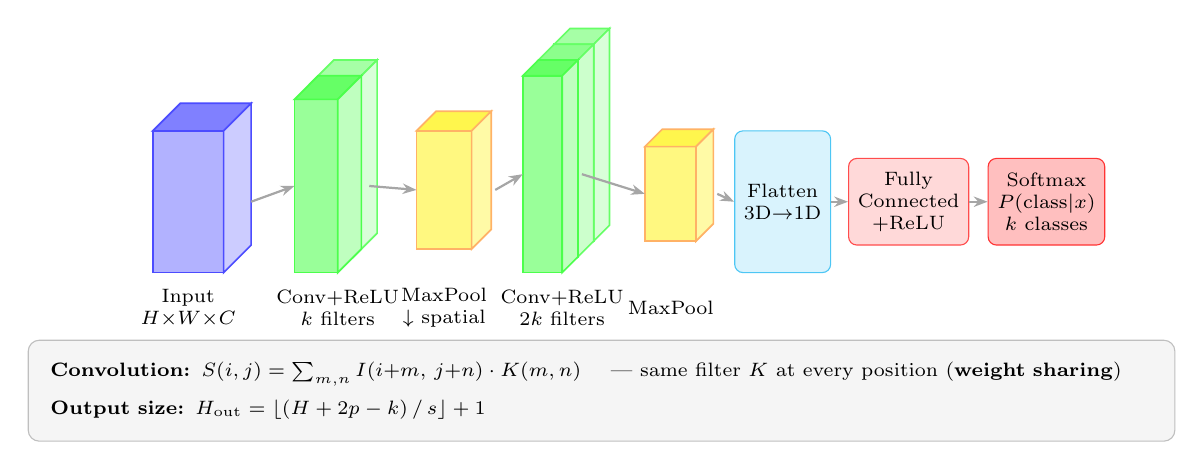
\begin{tikzpicture}[
  every node/.style={font=\small},
  arr/.style={-{Stealth[length=5pt]}, thick, gray!70},
  lbl/.style={font=\scriptsize, align=center}
]

%% Helper macro: draw a 3D block volume
%% Args: anchor-name, x, y, width, height, depth, fill-color, label
%% Front face, top face, right side face

% ---------- Input block (blue) ----------
\def\bx{0} \def\by{0}
\def\bw{0.9} \def\bh{1.8} \def\bd{0.35}
\fill[blue!30, draw=blue!70, line width=0.6pt]
  (\bx,\by) rectangle (\bx+\bw, \by+\bh);                        % front
\fill[blue!50, draw=blue!70, line width=0.6pt]
  (\bx,\by+\bh) -- (\bx+\bd,\by+\bh+\bd) -- (\bx+\bw+\bd,\by+\bh+\bd) -- (\bx+\bw,\by+\bh) -- cycle; % top
\fill[blue!20, draw=blue!70, line width=0.6pt]
  (\bx+\bw,\by) -- (\bx+\bw+\bd,\by+\bd) -- (\bx+\bw+\bd,\by+\bh+\bd) -- (\bx+\bw,\by+\bh) -- cycle; % right
\node[lbl, align=center] at (\bx+\bw/2, \by-0.45) {Input\\$H{\times}W{\times}C$};

% ---------- Conv+ReLU 1 (green, 2-layer stack) ----------
\def\cx{1.8}
% layer 2 (back, offset)
\fill[green!20, draw=green!60, line width=0.6pt]
  (\cx+0.2, 0.2) rectangle (\cx+0.2+0.55, 0.2+2.2);
\fill[green!35, draw=green!60, line width=0.6pt]
  (\cx+0.2, 0.2+2.2) -- (\cx+0.2+0.3, 0.2+2.2+0.3) -- (\cx+0.2+0.55+0.3, 0.2+2.2+0.3) -- (\cx+0.2+0.55,0.2+2.2) -- cycle;
\fill[green!15, draw=green!60, line width=0.6pt]
  (\cx+0.2+0.55,0.2) -- (\cx+0.2+0.55+0.3,0.2+0.3) -- (\cx+0.2+0.55+0.3,0.2+2.2+0.3) -- (\cx+0.2+0.55,0.2+2.2) -- cycle;
% layer 1 (front)
\fill[green!40, draw=green!70, line width=0.6pt]
  (\cx, 0) rectangle (\cx+0.55, 2.2);
\fill[green!60, draw=green!70, line width=0.6pt]
  (\cx, 2.2) -- (\cx+0.3,2.2+0.3) -- (\cx+0.55+0.3,2.2+0.3) -- (\cx+0.55,2.2) -- cycle;
\fill[green!25, draw=green!70, line width=0.6pt]
  (\cx+0.55,0) -- (\cx+0.55+0.3,0.3) -- (\cx+0.55+0.3,2.2+0.3) -- (\cx+0.55,2.2) -- cycle;
\node[lbl] at (\cx+0.55, -0.45) {Conv+ReLU\\$k$ filters};

% ---------- MaxPool 1 (yellow) ----------
\def\mx{3.35}
\fill[yellow!50, draw=orange!60, line width=0.6pt]
  (\mx,0.3) rectangle (\mx+0.7, 1.8);
\fill[yellow!70, draw=orange!60, line width=0.6pt]
  (\mx,1.8) -- (\mx+0.25,1.8+0.25) -- (\mx+0.7+0.25,1.8+0.25) -- (\mx+0.7,1.8) -- cycle;
\fill[yellow!35, draw=orange!60, line width=0.6pt]
  (\mx+0.7,0.3) -- (\mx+0.7+0.25,0.3+0.25) -- (\mx+0.7+0.25,1.8+0.25) -- (\mx+0.7,1.8) -- cycle;
\node[lbl] at (\mx+0.35, -0.45) {MaxPool\\$\downarrow$ spatial};

% ---------- Conv+ReLU 2 (green, 3-layer stack, taller) ----------
\def\cx{4.7}
% layer 3 (back)
\fill[green!20, draw=green!60, line width=0.6pt]
  (\cx+0.4, 0.4) rectangle (\cx+0.4+0.5, 0.4+2.5);
\fill[green!35, draw=green!60, line width=0.6pt]
  (\cx+0.4,0.4+2.5) -- (\cx+0.4+0.2,0.4+2.5+0.2) -- (\cx+0.4+0.5+0.2,0.4+2.5+0.2) -- (\cx+0.4+0.5,0.4+2.5) -- cycle;
\fill[green!15, draw=green!60, line width=0.6pt]
  (\cx+0.4+0.5,0.4) -- (\cx+0.4+0.5+0.2,0.4+0.2) -- (\cx+0.4+0.5+0.2,0.4+2.5+0.2) -- (\cx+0.4+0.5,0.4+2.5) -- cycle;
% layer 2 (middle)
\fill[green!30, draw=green!60, line width=0.6pt]
  (\cx+0.2, 0.2) rectangle (\cx+0.2+0.5, 0.2+2.5);
\fill[green!45, draw=green!60, line width=0.6pt]
  (\cx+0.2,0.2+2.5) -- (\cx+0.2+0.2,0.2+2.5+0.2) -- (\cx+0.2+0.5+0.2,0.2+2.5+0.2) -- (\cx+0.2+0.5,0.2+2.5) -- cycle;
\fill[green!20, draw=green!60, line width=0.6pt]
  (\cx+0.2+0.5,0.2) -- (\cx+0.2+0.5+0.2,0.2+0.2) -- (\cx+0.2+0.5+0.2,0.2+2.5+0.2) -- (\cx+0.2+0.5,0.2+2.5) -- cycle;
% layer 1 (front)
\fill[green!40, draw=green!70, line width=0.6pt]
  (\cx, 0) rectangle (\cx+0.5, 2.5);
\fill[green!60, draw=green!70, line width=0.6pt]
  (\cx,2.5) -- (\cx+0.2,2.5+0.2) -- (\cx+0.5+0.2,2.5+0.2) -- (\cx+0.5,2.5) -- cycle;
\fill[green!25, draw=green!70, line width=0.6pt]
  (\cx+0.5,0) -- (\cx+0.5+0.2,0.2) -- (\cx+0.5+0.2,2.5+0.2) -- (\cx+0.5,2.5) -- cycle;
\node[lbl] at (\cx+0.5, -0.45) {Conv+ReLU\\$2k$ filters};

% ---------- MaxPool 2 (yellow) ----------
\def\mx{6.25}
\fill[yellow!50, draw=orange!60, line width=0.6pt]
  (\mx,0.4) rectangle (\mx+0.65, 1.6);
\fill[yellow!70, draw=orange!60, line width=0.6pt]
  (\mx,1.6) -- (\mx+0.22,1.6+0.22) -- (\mx+0.65+0.22,1.6+0.22) -- (\mx+0.65,1.6) -- cycle;
\fill[yellow!35, draw=orange!60, line width=0.6pt]
  (\mx+0.65,0.4) -- (\mx+0.65+0.22,0.4+0.22) -- (\mx+0.65+0.22,1.6+0.22) -- (\mx+0.65,1.6) -- cycle;
\node[lbl] at (\mx+0.33, -0.45) {MaxPool};

% ---------- Flatten (light blue) ----------
\node[draw=cyan!70, fill=cyan!15, rounded corners=3pt, minimum width=1.1cm, minimum height=1.8cm,
      align=center, font=\scriptsize] (flat) at (8.0, 0.9) {Flatten\\3D$\to$1D};

% ---------- FC (red) ----------
\node[draw=red!70, fill=red!15, rounded corners=3pt, minimum width=1.2cm, minimum height=1.1cm,
      align=center, font=\scriptsize] (fc) at (9.6, 0.9) {Fully\\Connected\\+ReLU};

% ---------- Softmax (red) ----------
\node[draw=red!80, fill=red!25, rounded corners=3pt, minimum width=1.3cm, minimum height=1.1cm,
      align=center, font=\scriptsize] (sm) at (11.35, 0.9) {Softmax\\$P(\text{class}|x)$\\$k$ classes};

% ---------- Arrows ----------
% Input -> Conv1
\draw[arr] (0.9+0.35, 0.9) -- (1.8, 1.1);
% Conv1 -> MaxPool1
\draw[arr] (1.8+0.55+0.3+0.1, 1.1) -- (3.35, 1.05);
% MaxPool1 -> Conv2
\draw[arr] (3.35+0.7+0.25+0.05, 1.05) -- (4.7, 1.25);
% Conv2 -> MaxPool2
\draw[arr] (4.7+0.5+0.2+0.05, 1.25) -- (6.25, 1.0);
% MaxPool2 -> Flatten
\draw[arr] (6.25+0.65+0.22+0.05, 1.0) -- (flat.west);
% Flatten -> FC
\draw[arr] (flat.east) -- (fc.west);
% FC -> Softmax
\draw[arr] (fc.east) -- (sm.west);

% ---------- Formula box ----------
\node[draw=gray!50, fill=gray!8, rounded corners=4pt, align=left, font=\scriptsize,
      inner sep=8pt, text width=14cm] at (5.7, -1.5) {%
  \textbf{Convolution:} $S(i,j) = \sum_{m,n} I(i{+}m,\,j{+}n)\cdot K(m,n)$ \quad
  --- same filter $K$ at every position (\textbf{weight sharing})\\[4pt]
  \textbf{Output size:} $H_{\text{out}} = \left\lfloor (H + 2p - k) \,/\, s \right\rfloor + 1$
};

\end{tikzpicture}

\end{document}
